% Manuscript-ready section; counts describe the supplied workbooks with the
% default QC threshold (24 unique points). Recheck counts if data or QC changes.
% Required packages: booktabs, graphicx, url.
% Paths are relative to the repository root, not this file's directory.
% Add dataset_references.bib to the manuscript's existing bibliography.

\section{Dataset and preprocessing}
\label{sec:dataset}

\subsection{Data sources and study population}

We analyzed continuous glucose monitoring (CGM) data from the study of
Hall et al.~\cite{hall2018glucotypes}, using two supplied Excel workbooks:
\path{hall2018_full_another_version.xlsx} and
\path{pbio.2005143.s015.xlsx}. The original study used a Dexcom G4 sensor
with nominal five-minute sampling. The second workbook corresponds to the
standardized-meal supplement, designated \emph{S6 Data} in the original
publication~\cite{hall2018mealdata}; ``s015'' is its supplementary-file
identifier, not its dataset number. All sample sizes below were computed
from the supplied workbooks after auditing, rather than assumed from the
published study protocol.

The Hall workbook contains 105,417 CGM readings from 57 participants.
Participant identifiers, timestamps, glucose concentrations in mg/dL, age,
and glycemic-status labels are available. We use the supplied status coding
of 0, 0.5, and 2 to identify 38 normoglycemic participants (labeled
\emph{Healthy} in the workbook), 14 participants with prediabetes, and
5 participants with type 2 diabetes, respectively. These are the supplied
clinical-status groups, not the low-, moderate-, and severe-variability
``glucotypes'' investigated in the source study. We did not reclassify
participants using their meal-response curves. Age in the full cohort is
$48.9\pm13.8$ years (mean $\pm$ sample standard deviation; range 25--76).
The supplied extract contains 1,584--2,361 readings per participant
(median 1,822). Recording gaps are present; elapsed time between a
participant's first and last timestamps is therefore not interpreted as
continuous sensor wear time.

\subsection{Standardized meals and linkage}

The meal workbook contains 6,152 input rows from 30 participants, with
four fields: meal label, participant identifier, timestamp, and glucose
value. The three standardized breakfasts are bread with peanut butter
(PB), a PROBAR protein bar (Bar), and cornflakes with milk (CF), with
two intended repetitions of each meal~\cite{hall2018glucotypes}.
The labels PB~1/PB~2, Bar~1/Bar~2, and CF~1/CF~2 identify the meal type
and repetition. The specified observation window runs from 30 minutes
before the meal to 150 minutes afterward~\cite{hall2018mealdata}.

All 30 meal participants match a participant in the Hall workbook by
identifier. Their subgroup counts are 20 normoglycemic, 7 prediabetes,
and 3 type 2 diabetes; their mean age is $41.9\pm14.2$ years (range 25--65).
Thus, the meal data form a nested subset, not an independent validation
cohort. We link the files by participant identifier to obtain age and
status, without assuming that every meal timestamp is also present in
the supplied Hall extract. The two files are not concatenated to inflate
the number of independent observations. Table~\ref{tab:dataset-cohort}
summarizes the two analysis populations.

\begin{table}[htbp]
\centering
\caption{Composition of the supplied Hall2018 extract and its standardized-meal subset. Meal-window counts are after the present analysis's quality control. The meal subset is nested within the Hall cohort, not an independent dataset.}
\label{tab:dataset-cohort}
\small
\begin{tabular}{lrrrrrr}
\toprule
& Hall & Hall CGM & Meal & \multicolumn{3}{c}{Retained meal windows} \\
\cmidrule(lr){5-7}
Status & persons & readings & persons & PB & Bar & CF \\
\midrule
Normoglycemic & 38 & 70,527 & 20 & 36 & 32 & 33 \\
Prediabetes & 14 & 25,677 & 7 & 11 & 11 & 10 \\
Type 2 diabetes & 5 & 9,213 & 3 & 4 & 4 & 6 \\
\midrule
All participants & 57 & 105,417 & 30 & 51 & 47 & 49 \\
\bottomrule
\end{tabular}
\end{table}


\subsection{Quality control and time alignment}

A meal event is defined by a unique participant--meal-label pair.
The nominal design yields $30\times3\times2=180$ participant--meal slots;
176 have records in the supplied workbook and four are absent.
We first average records sharing the same participant, meal label, and
timestamp. This collapses 87 excess duplicate rows, leaving 6,065 unique
timestamped points before event exclusion. Six literal \texttt{Low}
readings are represented by 40~mg/dL as a numerical floor approximation,
not as exact measured concentrations. Points affected by duplicate
aggregation or this low-value substitution receive an observation weight
of 0.8 rather than 1 in parameter estimation. These are preprocessing
choices of the present analysis.

An event is retained if it has linked participant metadata, an observed
timestamp span of 180 minutes within a tolerance of 0.1 minute, and at
least 24 unique CGM points. Twenty-six events fail the span criterion
(eight also fail the point-count criterion); a further three have a full
span but fewer than 24 points. Consequently, 147 of the 176 observed
events are retained (83.5\%), and all 30 meal participants remain.
The retained events comprise 51 PB, 47 Bar, and 49 CF windows, with
3--6 windows per participant (median 5). By clinical-status group,
101, 32, and 14 windows belong to normoglycemia, prediabetes, and
type 2 diabetes, respectively.

For retained full-span windows, meal time is assigned to 30 minutes after
the first timestamp, following the supplement's stated window convention;
the workbook does not provide a separate meal-onset field. This yields a
relative-time axis of $[-30,150]$ minutes. There are 5,313 retained unique
CGM points: 861 strictly before the meal and 4,452 at or after $t=0$.
Each retained window contains 24--37 points (median 37). A full timestamp
span does not imply uninterrupted sampling: internal missing points can
remain, with the largest retained within-window gap being 55 minutes.
The event-level inclusion decisions are preserved in the QC table.
Figure~\ref{fig:dataset-overview} displays cohort nesting, exclusion counts,
and coverage for every participant and meal repetition.

\begin{figure}[htbp]
\centering
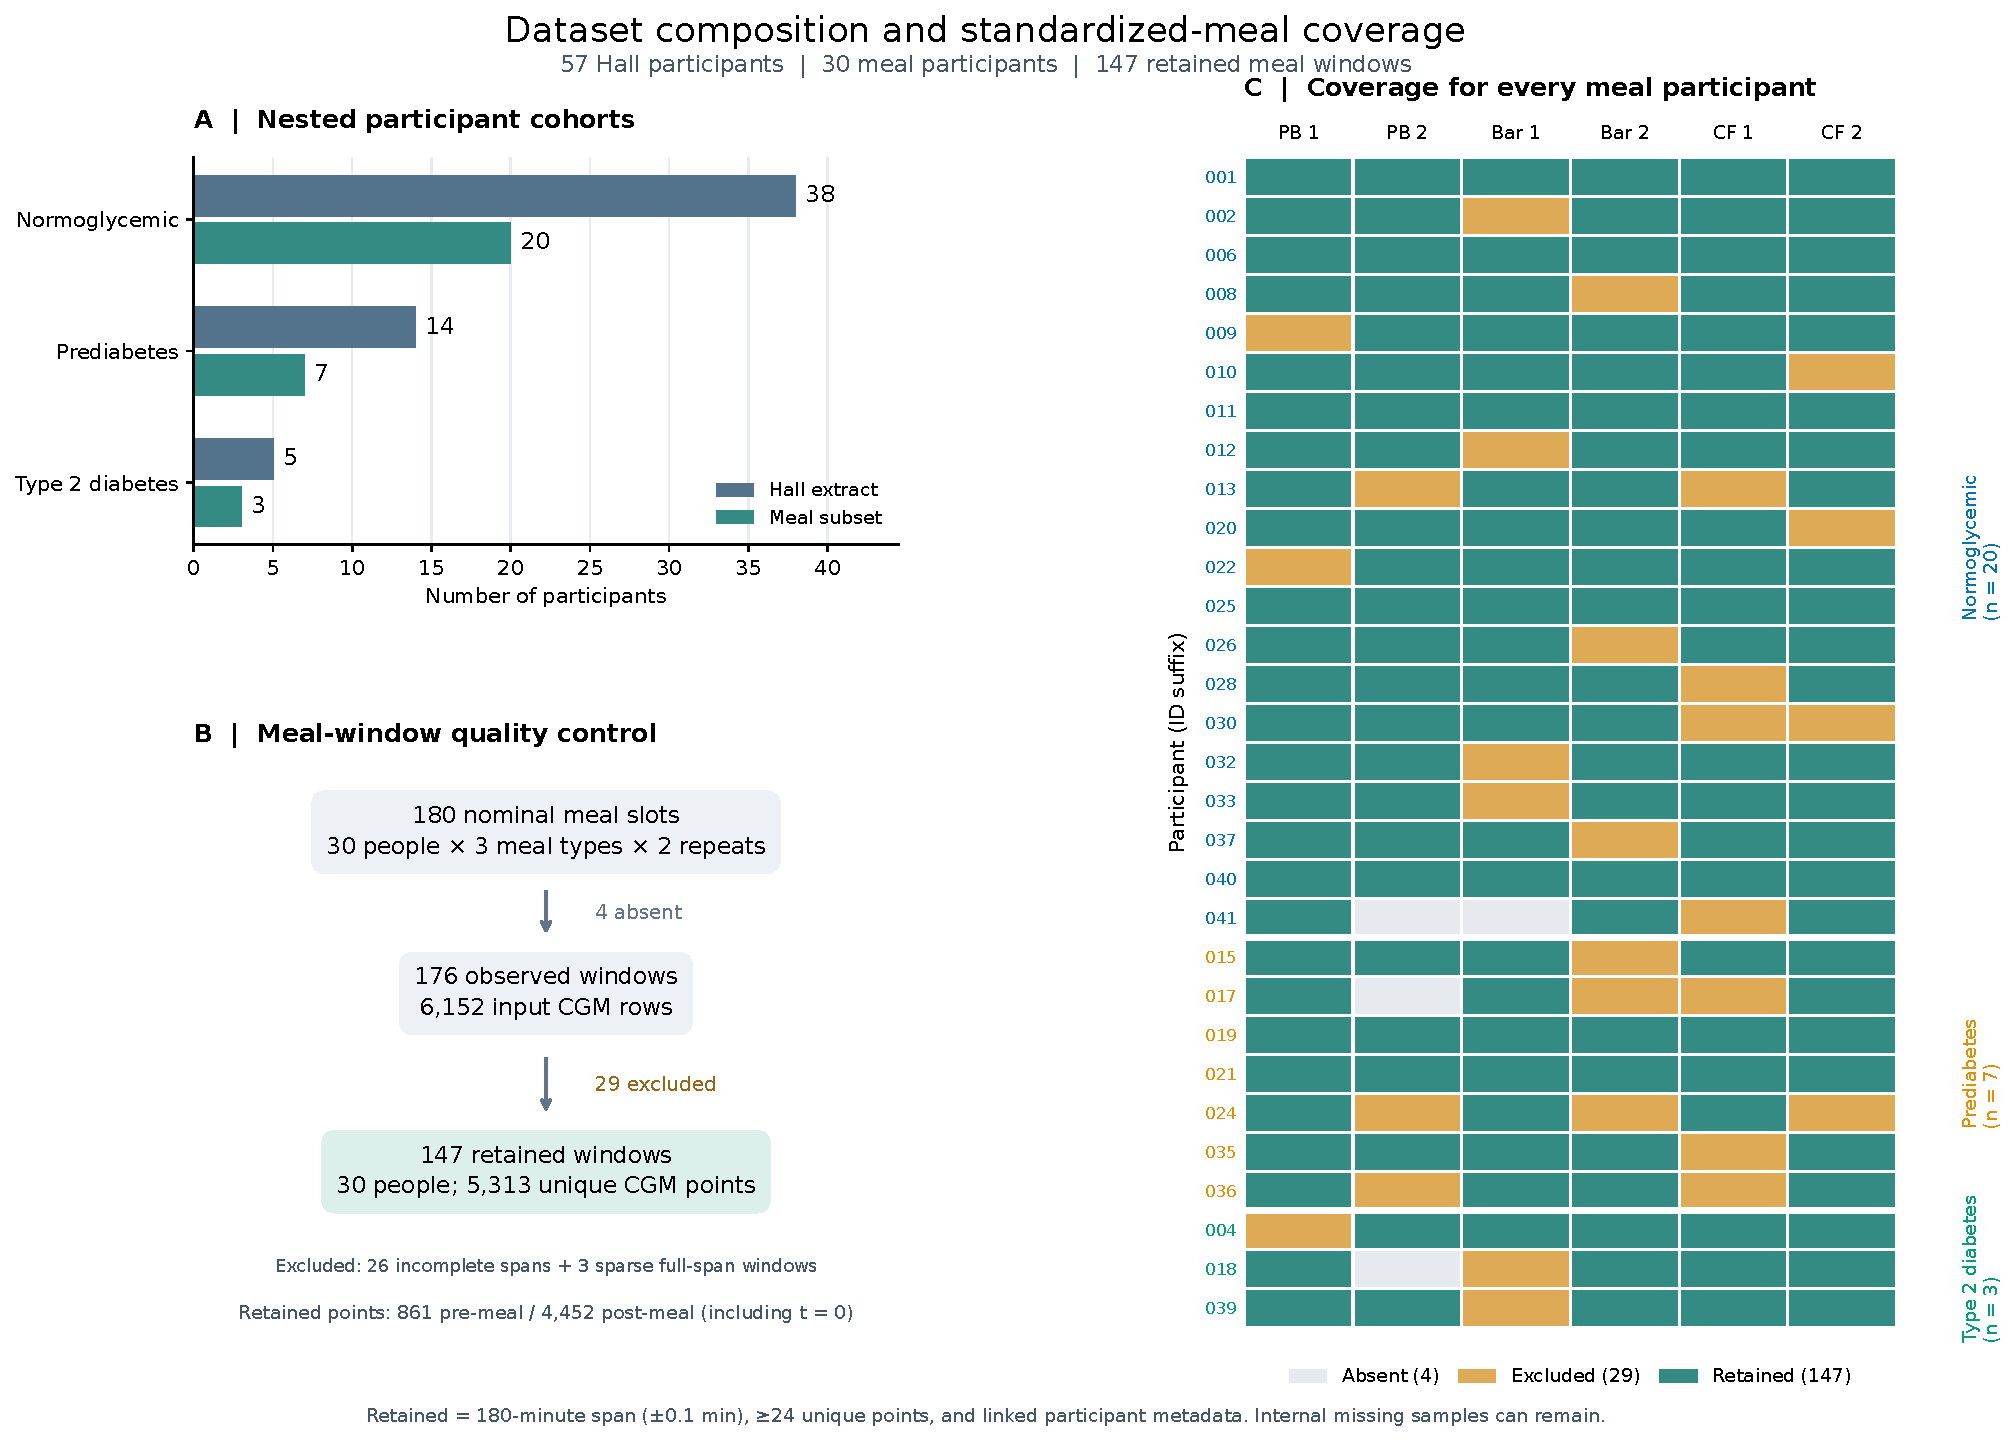
\includegraphics[width=\linewidth]{outputs/figures/figure_6_dataset_overview.pdf}
\caption{Composition and coverage of the supplied dataset.
(A) Participant counts in the Hall extract and its nested meal subset.
(B) Accounting of nominal slots, observed windows, and windows retained
under the present QC criteria. The 26 incomplete-span exclusions include
eight windows that also have fewer than 24 unique points; the three
sparse full-span windows are additional exclusions.
(C) Availability of each of the six intended meal repetitions for every
meal participant. Gray denotes an absent slot, amber an observed but
excluded window, and teal a retained window. Rows are grouped by the
supplied glycemic-status labels; participant labels are study-ID suffixes.
Retention does not imply that all internal samples are present.}
\label{fig:dataset-overview}
\end{figure}

\subsection{Descriptive profiles and analytical scope}

For the descriptive meal-response figure, available repetitions of a meal
type are first averaged within each participant at each relative time.
These participant-level values are then averaged within each clinical-status
group, giving equal weight to each contributing participant rather than to
each meal repetition. Shading represents pointwise 95\% bootstrap confidence
intervals for the group mean, not the spread of individual responses.
No missing values are imputed for this visualization; therefore, the
number of contributing participants can vary over time. The curves show
absolute CGM concentrations and consequently reflect both pre-meal glucose
differences and postprandial excursions. They are intended as an exploratory
description, not as a test of group separation, a causal comparison of
meal types, or evidence of model or controller efficacy.

The Hall extract supports cohort description and supplies participant
metadata. The retained meal windows support individualized dynamic-model
estimation: observations at $t\geq0$ enter the dynamical fitting loss,
whereas pre-meal observations supply reference-glucose information.
Repeated meals are nested within participants and are not independent
subjects. The current control experiment uses one simulated scenario per
fitted participant, not an observed treatment trial or 147 independent
control evaluations. Neither of the two supplied workbooks includes
measured insulin concentrations or administered insulin doses; sex and
insulin-modality fields in the Hall workbook are entirely missing.
These limitations concern the selected files, not all measurements
collected in the original study. The small and imbalanced meal subset,
especially its three participants with type 2 diabetes, residual sampling
gaps, and the absence of an independent validation cohort limit the
generalizability of subgroup and model-based conclusions.
